\section{Introduction}

The information age is driven by data stored in ever-growing relational databases and data warehouses 
that have come to underpin nearly all technology stacks. Data warehouses typically store information in multiple tables, with entities/rows in different tables connected using primary-foreign key relations, and managed using powerful query languages such as SQL \citep{codd1970relational,chamberlin1974sequel}. For this reason, data warehouses underpin many of today's large information systems, including e-commerce, social media, banking systems, healthcare, manufacturing, and open-source scientific knowledge repositories~\citep{johnson2016mimic,pubmed}.


Many predictive problems over relational data have significant implications for human decision making. A hospital wants to predict the risk of discharging a patient; an e-commerce company wishes to forecast future sales of each of their products; a telecommunications provider wants to predict which customers will churn; and a music streaming platform must decide which songs to recommend to a user. Behind each of these tasks is a rich relational schema of relational tables, and many machine learning models are built using this data~\citep{kaggle-survey}. 

However, existing learning paradigms, notably tabular learning, cannot be directly applied to an interlinked set relational tables.
Instead, a manual feature engineering step is first taken, where a data scientist uses domain knowledge to manually join and aggregate tables to generate many features in a regular single table format. 
To illustrate this, consider a simple e-commerce schema (Fig. \ref{fig: high level outline (fig1)}) of three tables: \tbl{Customers}, \tbl{Transactions} and \tbl{Products}, where \tbl{Customers} and \tbl{Products} tables link into the \tbl{Transactions} table via primary-foreign keys, and the task is to predict if a customer is going to churn (\emph{i.e.}, make zero transactions in the next $k$ days). In this case, the data scientist would aggregate information from the \tbl{Transactions} table to make new features for the \tbl{Customers} table such as: ``number of purchases of a given customer in the last 30 days'', ``sum of purchase amounts of a given customer in the last 30 days'', ``number of purchases on a Sunday'', ``sum of purchase amounts on a Sunday'', ``number of purchases on a Monday'', and so on. The computed customer features are then stored in a single table, ready for tabular machine learning. Another challenge is the {\em temporal} nature of the churn predictive tasks. As new transactions appear, the customer's churn label and the customer's features may change from day to day, so features need to be recomputed for each day. Overall, the temporal nature of relational databases adds computational cost and further complexity, which often results in bugs and information leakage including the so-called ``time travel'' \citep{kapoor2023leakage}.


\begin{figure}[t] % 'h' for here
  \centering
  \begin{tikzpicture}

\node (ex1) at (5,0)
{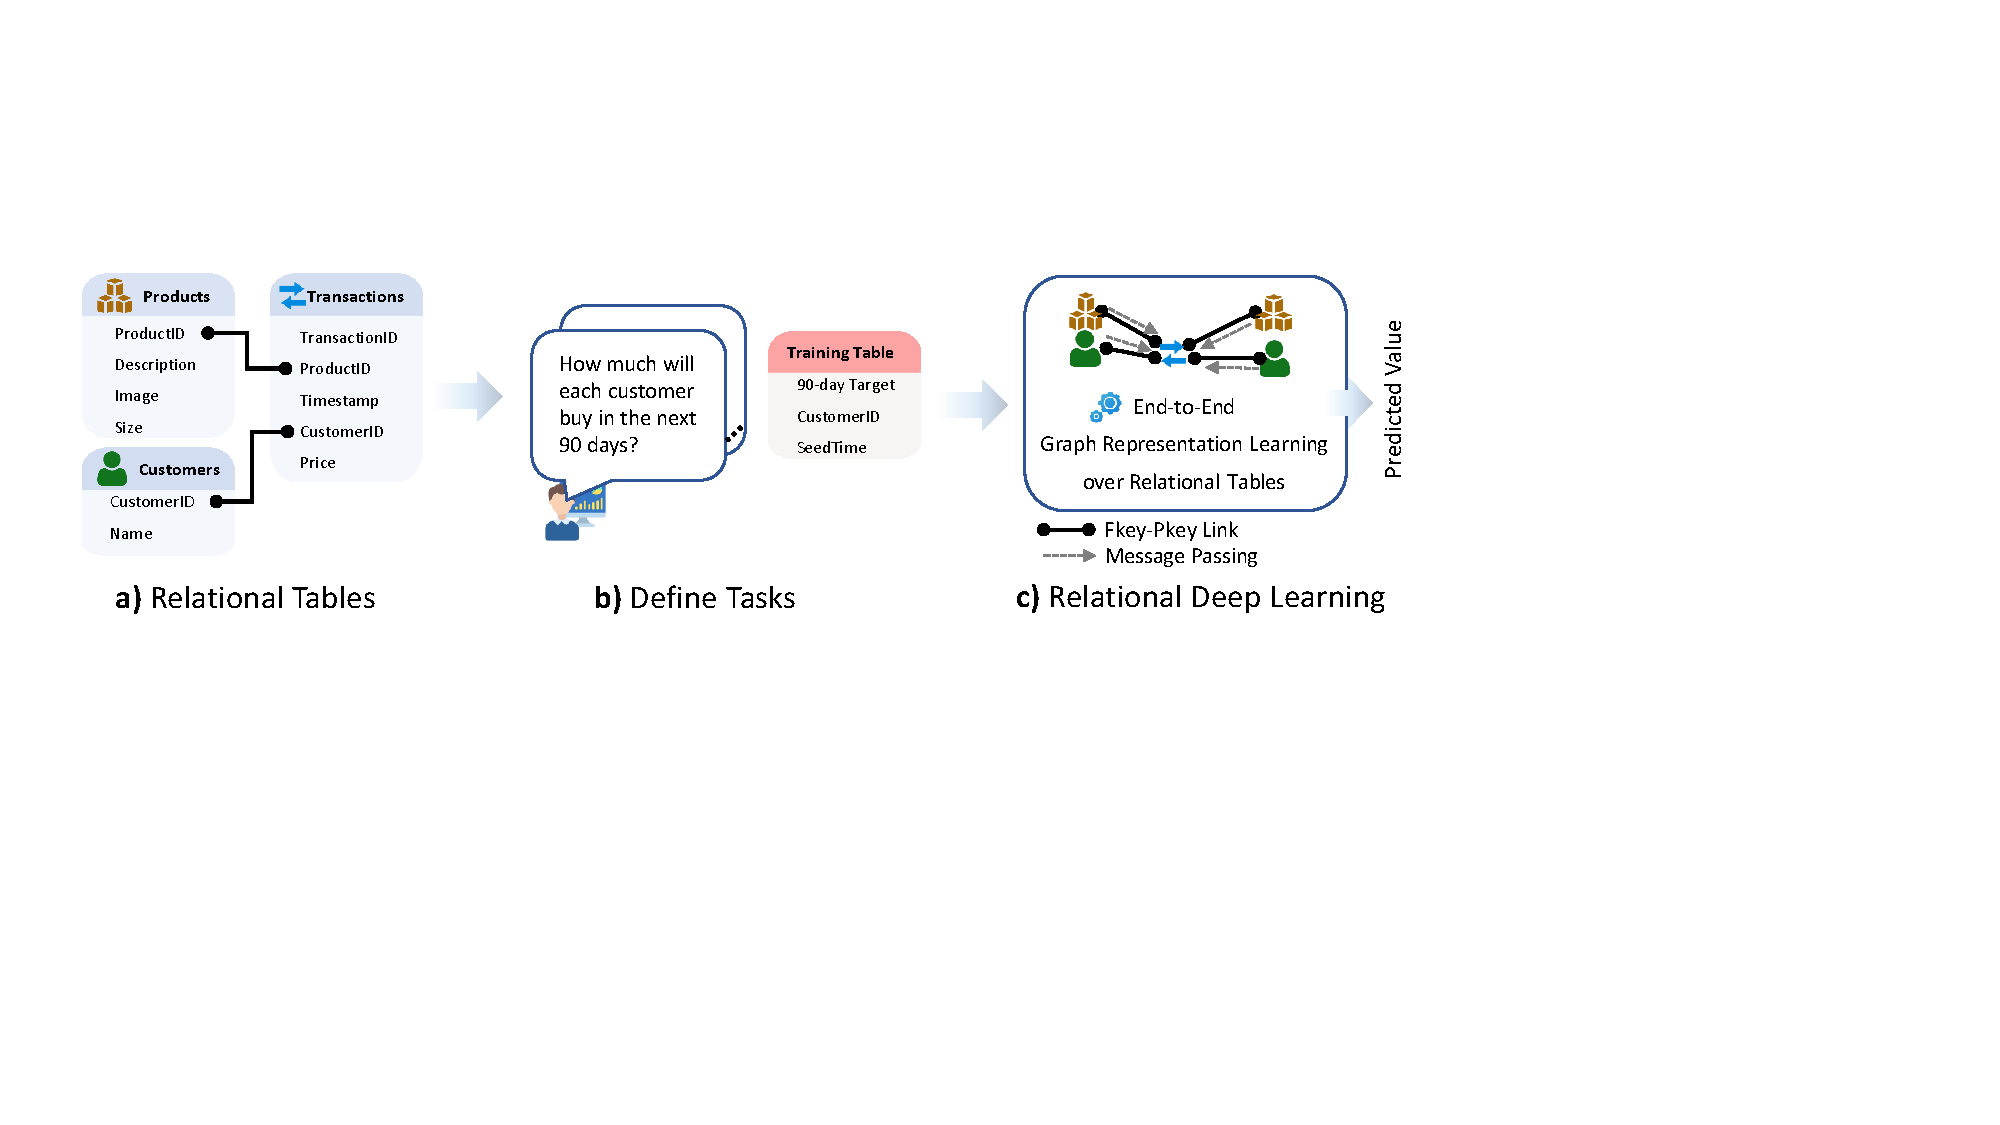
\includegraphics[trim={0.4cm 0.6cm 0cm 0cm}, clip, scale=0.62]{figs/f1_alt.pdf}};
\node[scale=0.8] at (-0.1,-1.8) { \textbf{(a)} Relational Database};

\node[scale=0.8] at (4.6,-1.8) { \textbf{(b)} Define Tasks};

\node[scale=0.8] at (9.5,-1.81) { \textbf{(c)} Relational Deep Learning};

\end{tikzpicture}
  \caption{\textbf{\AreaName solves predictive tasks on relational data with end-to-end learnable models.} There are three main steps. (a) A relational database with multiple tables connected by primary-foreign keys is given. (b) A predictive task is specified and added to the database by introducing an additional training table. (c) Relational data is transformed into its {\em Relational Entity Graph}, and a Graph Neural Network is trained over the graph with the supervision provided by the training table. The predictive task can be node level (as in this illustration), link level (pairs of nodes), or higher-order.}
  \label{fig: high level outline (fig1)}
\end{figure}


There are several issues with with the above approach: (1) it is a manual, slow and labor intensive process; (2) feature choices are essentially arbitrary and likely highly-suboptimal; 
%and the data scientists hopes that hand engineered features will be correlated with the label they aim to predict; 
(3) only a small fraction of the overall space of possible features can be manually explored; (4) by forcing data into a single table, information is aggregated into lower-granularity features, thus losing out on valuable fine-grain signal; (5) whenever the data distribution changes or drifts, current features become obsolete and new features have to be manually reinvented.


Many domains have been in a similar position, including pre-deep-learning computer vision, where hand-chosen convolutional filters  (\emph{e.g.}, Gabor) were used to extract features, followed by models such as SVMs or nearest neighbor search \citep{varma2005statistical}. Today, in contrast, deep neural networks skip the feature engineering and learn directly on the raw pixels, which results in large gains in model accuracy.
More broadly, the deep learning revolution has had a huge impact in many fields, including computer vision~\citep{he2016deep,russakovsky2015imagenet}, natural language processing~\citep{vaswani2017attention,devlin2018bert,brown2020language}, and speech~\citep{hannun2014deep,amodei2016deep}, and has led to super-human performance in many tasks. In all cases, the key was to move from manual feature engineering and handcrafted systems to fully data-driven, end-to-end representation learning systems.
For relational data, this transition has not yet occurred, as existing tabular deep learning approaches still heavily rely on manual feature engineering. 
Consequently, there remains a huge unexplored opportunity.


Here we introduce \emph{\AreaName (RDL)}, a blueprint for fulfilling the need for an end-to-end deep learning paradigm for relational tables (Fig. \ref{fig: high level outline (fig1)}).
Through end-to-end representation learning, \AreaName fully utilizes the rich predictive signals available in relational tables. The core of RDL is to represent relational tables as a temporal, heterogeneous  {\em Relational Entity Graph}, where each row defines a node, columns define node features, and primary-foreign key links define edges. Graph Neural Networks (GNNs)~\citep{gilmer2017mpgnn, hamilton2017inductive} can then be applied to build end-to-end data-driven predictive models.



Predictive tasks are specified on relational data by introducing a {\em training table} that holds supervision label information, (Fig. \ref{fig: high level outline (fig1)}b) but no input features. 
Training tables have two critically important characteristics. First, labels can be automatically computed from historical relational data, without any need for outside annotation; second, they may contain any number of foreign keys, permitting many task types including entity level (1 key, as in Fig. \ref{fig: high level outline (fig1)}b), link-level tasks such as recommendation (2 keys) and multi-entity tasks ($>$2 keys). Training tables permit many different types of prediction targets, including multi-class, multi-label, regression and more, ensuring high task generality.

All in all, RDL model pipeline has four main steps (Fig.~\ref{fig: end to end pipeline}): Given a predictive machine learning task, (1)  A \emph{training table} containing supervision labels is constructed in a task-specific manner based on historic data in the relational database, (2) entity-level features are extracted and encoded from each row in each table to serve as node features, (3) node representations are learned through an inter-entity message-passing GNN that exchanges information between entities with primary-foreign key links, (4) a task-specific model head produces predictions for training data, and errors are backpropogated through the network. 

\begin{figure}[t] % 'h' for here
  \centering
  \begin{tikzpicture}

\node (ex1) at (4.7,0)
{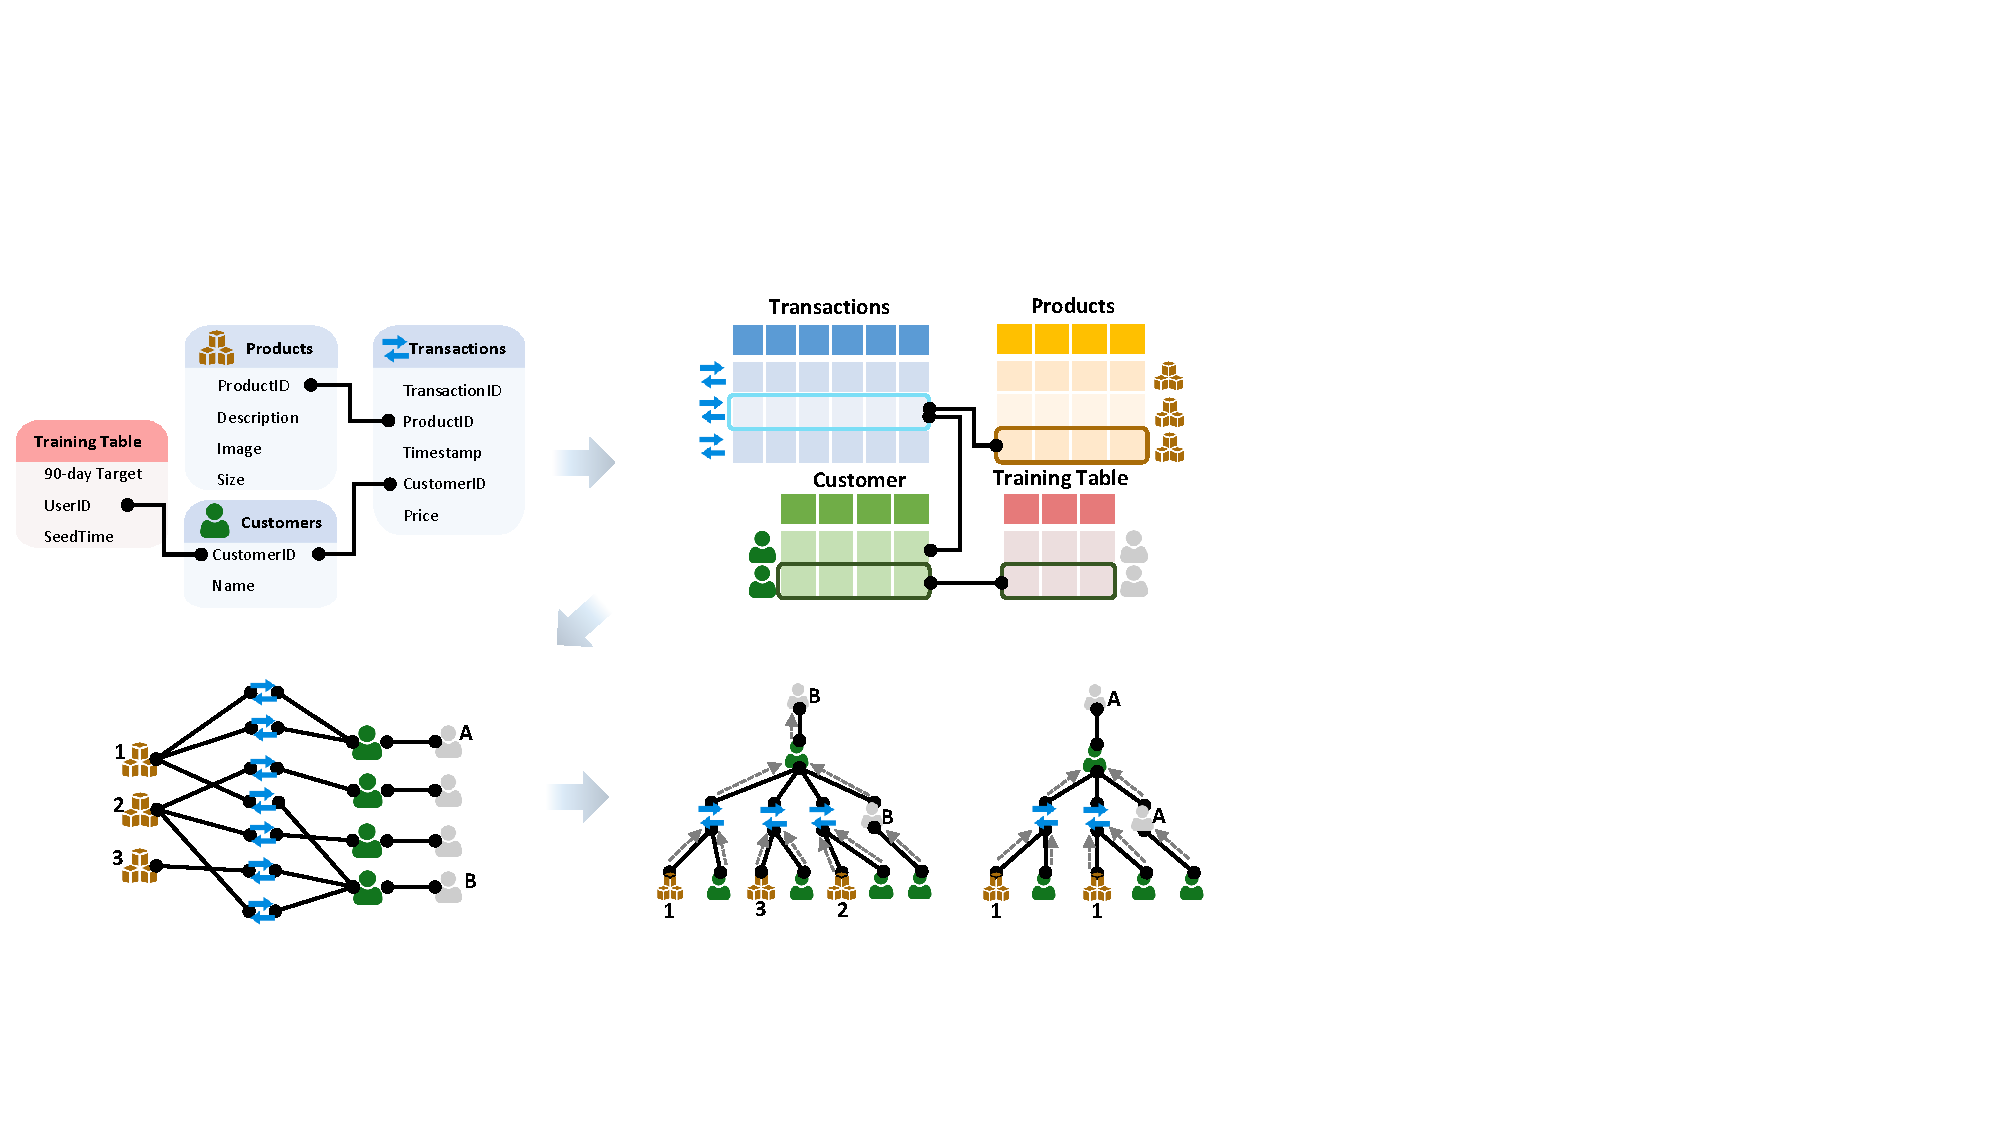
\includegraphics[trim={0cm 0cm 0cm 0cm}, clip, scale=0.67]{figs/f3_alt_2.pdf}};
\node[scale=0.8] at (1,-0.3) { \textbf{(a)} Rel. Tables with Training Table};

\node[scale=0.8] at (8.2,-0.3) { \textbf{(b)} Entities Linked by Foreign Keys};

\node[scale=0.8] at (1,-3.8) { \textbf{(c)} Relational Entity Graph};

\node[scale=0.8] at (8.2,-3.8) { \textbf{(d)} Graph Neural Network};

\end{tikzpicture}
  \caption{\textbf{Relational Deep Learning Pipeline.} \textbf{(a)} Given relational tables and a predictive task, a training table, containing supervised label information, is constructed and attached to the entity table(s). \textbf{(b)} Relational tables contain individual entities that are linked by foreign-primary key relations. \textbf{(c)} Relational data can be viewed as a single {\em Relational Entity graph}, which has a node for each entity, and edges given by primary-foreign key links. \textbf{(d)} Initial node features are extracted from each row in each table using modality-specific neural networks. Then a message passing graph neural network computes relation-aware node embeddings, a model head produces predictions for training table entities, and errors are backpropogated.
  }
  \label{fig: end to end pipeline}
\end{figure}

%% Jure commented this out. It feels like the issue of temporality
 Crucially, RDL models natively integrate temporality by only allowing entities to receive messages from other entities with earlier timestamps. This ensures that learned representation is automatically updated during GNN forward pass when new data is collected, and prevents information leakage and time travel bugs. Furthermore, this also stabilizes the generalization across time since models are trained to make predictions at multiple time snapshots by dynamically passing messages between entities at different time snapshots, whilst remaining grounded in a single relational database. 


\xhdr{\BenchmarkName} To facilitate research into \AreaName, we introduce {\em \BenchmarkName}, a benchmarking and an evaluation Python package. Data in \BenchmarkName cover rich relational databases from many different domains. \BenchmarkName has the following key modules (1) \textbf{Data:} data loading, specifying a predictive task, and (temporal) data splitting, (2) \textbf{Model:} transforming data to a heterogeneous graph, building graph neural network predictive models,  (3) \textbf{Evaluation:} standardized evaluation protocol given a file of predictions. Importantly, data and evaluation modules are deep learning framework agnostic, enabling broad compatibility. To facilitate research, we provide our initial model implementation based on PyTorch Frame~\citep{Hu_PyTorch_Frame_A_2023} for encoding table rows into input node embeddings, which is then processed by GNN models in PyTorch Geometric~\citep{fey2019fast} to update the embeddings via message passing over the relational entity graph.

For the initial release, \BenchmarkName contains two databases, each with two predictive tasks. The first database is from Stack Exchange, the question-answering website, and includes 7 tables such as posts, users, and votes. The predictive tasks are (1) to predict if a user is going to make a new contribution (post, answer etc.), and (2) to predict the popularity of a new question. The second database is a subset of the Amazon Product Catalog focusing on books. There are three tables: users, products, and reviews. The tasks are (1) to predict the lifetime value of a user, and (2) whether a user will stop using the site. 

  \iffalse
  \jure{can we change this example to be in line with our running example (H\&M schema).}
  \jure{Here we have 3 steps, in the introduction we say there are 4 steps.}
  \jure{it is unclear what those icons are and what do they refer to -- 3 cubes, thumbs up/down. Basically, use these icons also on the left where you define the schema.}
  \jure{I think traning table needs to appear as an extra table on the left. On the right training table is represented as a separate node labeled that then points to the right entity. Right now the problem is that training table appears on the bottom right and connects to a graph.\\
  Here is how to update the Fig.: left tower: remove the "Machine Learning" and "Prediction", replace that with the schema (from the top) and add the greem training table to the schema. Right tower show how we go from schema to the relational graph (which includes nodes from the data tables as well as the training table). Let me know if this makes sense.}
  \jure{Sec. 2 shoudl refer ot the "left tower" and Sec. 3 should refer to the panels of the ``right tower'' of Fig. 1. Step by step. If this makes the Fig. too big/detailed, we should perhaps split Fig 1 into two separate large Fig.s. One Fig. explains the graph creation. The other Fig. explains the GNN workflow.}
  \fi
  

Our objective is to establish deep learning on relational data as a new subfield of machine learning. We hope that this will be a fruitful research direction, with many opportunities for impactful ideas that make much better use of the rich predictive signal in relational data. This paper lays the ground for future work by making the following main sections:
\begin{itemize}
    \item \textbf{Blueprint.} {\em \AreaName}, an end-to-end learnable approach that ultilizes the predictive signals available in relational data, and supports temporal predictions.
    \item \textbf{Benchmarking Package} {\em \BenchmarkName}, an open-source Python package for benchmarking and evaluating GNNs on relational data. {\BenchmarkName} beta release introduces two relational databases, and specifies two prediction tasks for each. 
    \item \textbf{Research Opportunities.} Outlining a new research program for  \AreaName, including multi-task learning, new GNN architectures, multi-hop learning, and more.
\end{itemize}


\xhdr{Organization} Section \ref{sec: problem scope} provides background on relational tables and predictive task specification. 
Section \ref{sec:formal_rl_problem} introduces our central methodological contribution, a graph neural network approach to solving predictive tasks on relational data.
Section \ref{sec: benchmark} introduces {\em \BenchmarkName}, a new benchmark for relational tables, and standardized evaluation protocols. 
Section \ref{sec: new challenges} outlines a landscape of new research opportunities for graph machine learning on relational data. Finally, Section \ref{sec: related work} concludes by contextualizing our new framework within the tabular and graph machine learning literature.

